% !TEX encoding = UTF-8 Unicode
\chapter{Einleitung}
\markboth{1 Einleitung}{}

\section{Problemstellung}

Die Entscheidung über die Annahme von Kundenaufträgen unter Unsicherheiten hat weitreichenden Einfluss auf die Produktionsplanung und den Ertrag eines auftragsgesteuerten Fertigungsunternehmens. Ein solches Unternehmen der Auftragsfertigung steht vor dem Entscheidungsproblem, ob der Auftrag zur Produktion des Produkts wirtschaftlich ist. Die Anfragen treffen in beliebiger Reihenfolge ein und haben eine unterschiedliche Wertigkeit. Im weiteren Verlauf dieser Arbeit werden Unternehmen betrachtet, die als auftragsbezogene Dienstleistung das Instandsetzen von Produkten anbieten. Abhängig des eingehenden Kundenauftrags, indem der Zustand des Produkts beschrieben ist, durch den die notwendigen Prozessschritte zur Instandsetzung des Produkts abgeleitet werden können, generiert das Unternehmen unterschiedliche Erträge. Die Prozessschritte zur Instandsetzung des Produkts geben zusätzlich den notwendigen Ressourcenbedarf für die auszuführende Tätigkeit an, die notwendig sind um das Produkt in seinen ursprünglichen bzw. geforderten Zustand zu versetzen. Ressourcen zur Instandsetzung von Produkten können z. B. Material oder Personalstunden sein. Abhängig des möglichen Ertrags und des für den Auftrag notwendigen Ressourcenbedarf muss das produzierende Unternehmen die Entscheidung über Annahme oder Ablehnung des Kundenauftrags treffen. Sofern nur dieser einfache Fall betrachtet wird, bei dem nur der einzelne Kundenauftrag zur Auswahl steht und die Abarbeitung der Aufträge nach der Eingangsreihenfolge erfolgt, ist die Entscheidung für das Unternehmen einfach getroffen. Der Kundenauftrag wird angenommen, sofern die Kosten des Ressourceneinsatzes niedriger als der erziele Ertrag ist.
Sofern das Unternehmen eine begrenzte Ressourcenkapazität zur Instandsetzung der Güter besitzt, muss zusätzlich der absolute Ressourcenverbrauch des Auftrags für die Annahmeentscheidung geprüft werden. Mit Annahme des Auftrags ist ein auftragsbezogener Ertrag erzielt und ein produktbezogener Ressourcenverbrauch eingetreten. Nachdem diese Entscheidung getroffen ist, wird der zeitlich nachfolgende Kundenauftrag betrachtet. Es handelt sich damit um ein klassisches Verfahren des \glqq First-come, first-served (FCFS){\grqq}.

Für die Entscheidung über die Annahme oder Ablehnung eines Kundenauftrags zur Instandhaltung von Produkten bedarf es einer umfassenderen Betrachtung, als nur die kurzsichtige Entscheidung über die Annahme einzelner Aufträge. Angenommen ein Unternehmen der Instandhaltung besitzt ein bestimmtes Kontingent an unterschiedlichen Ressourcen über einen bestimmten Zeitraum zur Erfüllung seiner angebotenen Dienstleistung. In diesem betrachteten Zeitraum treffen differenzierte Kundenaufträge mit unterschiedlicher Wertigkeit ein. Zur Maximierung der Erträge über den Betrachtungszeitraum kann es für das Unternehmen sinnvoll sein, Aufträge mit niedrigem Ertrag abzulehnen, sofern im weiteren Verlauf des betrachteten Zeitraums Aufträge mit höherem Ertrag eintreffen. Eine solche Entscheidung erfolgt in Abhängigkeit der noch vorhanden knappen Ressourcenkapazität, die für die unterschiedlichen Kundenaufträge aufgewendet werden müssen.

Eine weitere Alternative wäre es für das instandhaltende Unternehmen, das zu reparierende Produkt mit einem neuwertigen Produkt auszutauschen. Es handelt sich damit um eine Entscheidung der Lagerhaltung bei auftragsbezogenen Instandhaltungsprozessen. Die Entscheidung zur Reduzierung des vorhandenen Lagerbestands zur Befriedung von aktuellen Kundenaufträgen macht vor allem Sinn, wenn die zur Produktion notwendigen Ressourcen für spätere Aufträge notwendig sind. Für eine solche Entscheidung zur Befriedigung von aktuellen Aufträgen muss ein Lagerbestand der geforderten Produkte aufgebaut werden. Dabei steht im Mittelpunkt einer solchen Politik die optimale Kapazitätsauslastung und eine Ertragsmaximierung.

Auch unter solcher Entscheidungsalternativen kann zwischen dem einfachen Verfahren des FCFS und eines differenzierten Verfahrens unter Berücksichtigung von zukünftigen Fertigungsaufträgen unterschieden werden. Die kurzfristige Sichtweise untersucht nur den notwendigen Kapazitätsaufwand und den möglichen Ertrag des aktuellen Auftrags. Bei der langfristigen Sichtweise unter Berücksichtigung von zukünftigen Anfragen werden die vorhandenen Ressourcenkapazitäten und der Lagerbestand über einen längeren Zeitraum betrachtet. Sofern in der nahen Zukunft viele Aufträge eintreffen, muss ein solches langfristiges Verfahren eine Entscheidungsunterstützung dem Unternehmen liefern, ob eine Lagerproduktion zur Erhöhung des Lagerbestands erfolgen soll. Wie die Bezeichnung der Entscheidung zur Lagerproduktion bereits im Wortlauf deutlich macht, werden die durch den Ressourcenverbrauch geformten Leistungsbündel (Produkte) auf Lager produziert. Damit ist es dem Unternehmen möglich zu einem späteren Zeitpunkt die Anfragen mittels des Lagerbestands zu befriedigen.

\begin{figure}[h!]
  \begin{center}
    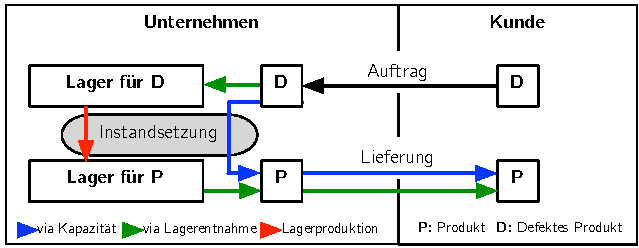
\includegraphics[width=120mm]{Bilder/Konzept.pdf}
    \caption{Grafische Darstellung der möglichen Entscheidung zur Befriedigung von auftragsbezogenen Instandhaltungsprozessen}  \label{Konzept}
  \end{center}
\end{figure}

In dieser Arbeit werden die in der Abbildung \ref{Konzept} möglichen Entscheidung zur Befriedigung von auftragsbezogenen Instandhaltungsprozessen betrachtet. Der Kunde kann innerhalb eines vordefinierten Buchungszeitraums einen Auftrag zur Instandsetzung eines defekten Produkts stellen. Sofern das Unternehmen einen solchen Auftragseingang erhält und sich für die \glqq Auftragsannahme via Kapazität{\grqq} entscheidet, wird der Auftrag über die vorhandene Produktions- bzw. Ressourcenkapazität abgewickelt. Alternativ kann das Unternehmen einen solchen Kundenauftrag auch durch einen Austausch des defekten mit einem neuwertigen Produkt befriedigen. D. h. das vom Kunden bereitgestellte defekte Produkt wird in ein Lager für defekte Produkt überführt und das Unternehmen liefert ein neuwertiges Produkt an den Kunden. Das neuwertige Produkt wird dabei aus einem Lager entnommen, dass für solche Produkte bereitgestellte ist. Diese Entscheidung wird als \glqq Auftragsannahme via Lagerentnahme{\grqq} bezeichnet. Weiter gibt es die Entscheidung, dass die Ressourcenkapazität für die Instandsetzung von defekten Produkten aus dem unternehmerischen Lager eingesetzt wird. D. h. ein defektes Produkt wird aufgearbeitet und dem Lager für neuwertige Produkte bereitgestellt. Damit ist ein neuer Lagerbestand an einem neuwertigen Produkt vorhanden und kann für nachfolgende Produktanfragen Verwendung finden. Die Entscheidung wird als \glqq Lagerproduktion{\grqq} bezeichnet und kann unabhängig eines Auftragseingangs erfolgen. Sofern jedoch diese Entscheidung aufgrund eines Auftragseingangs einer unrentablen Produktanfrage getroffen wird, handelt es dementsprechend um die Ablehnung der Produktanfrage. In dieser Arbeit wird angenommen, dass ein ausreichender Lagerbestand an defekten Produkten vorhanden ist, damit sämtliche Ressourcenkapazität für eine jeweilige Lagerproduktion eingesetzt werden kann. Daher wird der Bestand an defekten Produkten im weiteren Verlauf der Arbeit nicht betrachtet. Damit stehen dem Unternehmen in Summe die Entscheidungen \glqq Auftragsannahme via Kapazität{\grqq}, \glqq Auftragsannahme via Lagerentnahme{\grqq} und \glqq Lagerproduktion{\grqq} sowie die generelle \glqq Ablehnung der Anfrage{\grqq} zur Verfügung.

\section{Zielsetzung}

In dieser Arbeit wird ein mathematisches Modell für Annahmeentscheidungen von Aufträgen zur Instandsetzung von Produkten dargestellt. Dabei entspricht das durch den Instandhaltungsprozess reparierte Produkt den vom jeweiligen Auftrag geforderten Zustand. Das Modell berücksichtigt dabei die Entscheidungsmöglichkeit über die Auftragsannahme durch die Instandsetzung des Produkts mittels der verfügbaren Ressourcenkapazitäten oder die Befriedigung des Kundenauftrags durch Bereitstellung eines bereits reparierten Produkts. Dabei wird die Entscheidung der Bereitstellung des reparierten Produkts in Abhängigkeit des verfügbaren Lagerbestandes an neuwertigen Produkten getroffen.

Bei der in dieser Arbeit beschriebenen Modellformulierung des Auftragsannahmeproblems bei auftragsbezogenen Instandhaltungsprozessen handelt es sich um ein dynamisch, stochastisches Optimierungsmodell auf Basis des Konzepts des Netzwerk Revenue Managements. Das Optimierungsmodell trifft die Entscheidung, welche Entscheidung die optimale Politik des Auftragsannahmeproblems ist. Dabei ist die optimale Politik die Entscheidung die den möglichen Erwartungswert maximiert. Die Entscheidung erfolgt in Abhängigkeit der Veränderung der verfügbaren Ressourcenkapazitäten nach einer möglichen Instandsetzung des Produkts, des aktuell-vorhandenen Lagerbestandes der bereits reparierten Produkte und der noch potentiell eintreffenden Anfragen im Betrachtungszeitraum.

Das Revenue Management (RM) hat seinen Ursprung in der betrieblichen Problemstellung der Annahme von Aufträgen von freien Sitzplätzen in Passagierflugzeugen.\footnote{Vgl. \cite{talluri2004theory}, S. 6-10.} Das Grundmodell wird zur Annahme von Kundenaufträgen bzw. -anfragen von Dienstleistungsunternehmen mit beschränkten Ressourcenkapazitäten verwendet.\footnote{Vgl. \cite{Petrick:2009aa}, S. 182-187.} %kommt aus der wissenschaftlichen Betrachtung des Revenue Management .
Beim RM wird das Auftragsannahmeproblem der zeitlich nacheinander eintreffenden Produktanfragen als \textit{dynamisch, stochastisches Optimierungsmodell} formulieren und gelöst.
Die Aufgabe des Optimierungsmodells ist laut \cite{talluri2004theory} die Entscheidungsfindung zu unterstützen, damit der Gesamtertrag des Dienstleisters maximiert wird. Mit der Entscheidungsunterstützung ist die optimale Politik der Auftragsannahme für das betrachtete Netzwerk gemeint. Der Gesamtertrag wird in Geldeinheiten (GE) bewertet. 

%Bei den betrachteten Ressourcen handelt es sich um zeitgebundene Ressourcen mit einer jeweiligen vordefinierten Ressourcenkapazität über den gesamten Zeithorizont. 

Die Zielsetzung der Arbeit ist demnach das Grundmodell des Netzwerk RM zur Annahme von Kundenaufträgen mit der Möglichkeit der Berücksichtigung von Lagerhaltungsentscheidungen für auftragsbezogene Instandhaltungsprozesse zu erweitern. Zusätzlich zur konzeptionellen Darstellung des hier betrachteten Auftragsannehmeproblems wird für die Modellerweiterung ein Algorithmus entwickelt und implementiert, welches vorformulierte Beispielszenarien exakt löst. Anschließend wird eine numerische Untersuchung für mehrere Szenarien durchgeführen und die daraus resultierende optimale Politik untersucht. Damit wird dargestellt, welche Möglichkeiten sich für Unternehmen ergeben, sofern Lagerhaltungsentscheidungen bei auftragsbezogenen Instandhaltungsprozessen berücksichtigt werden.

\section{Aufbau der Arbeit}

\begin{figure}[h!]
  \begin{center}
    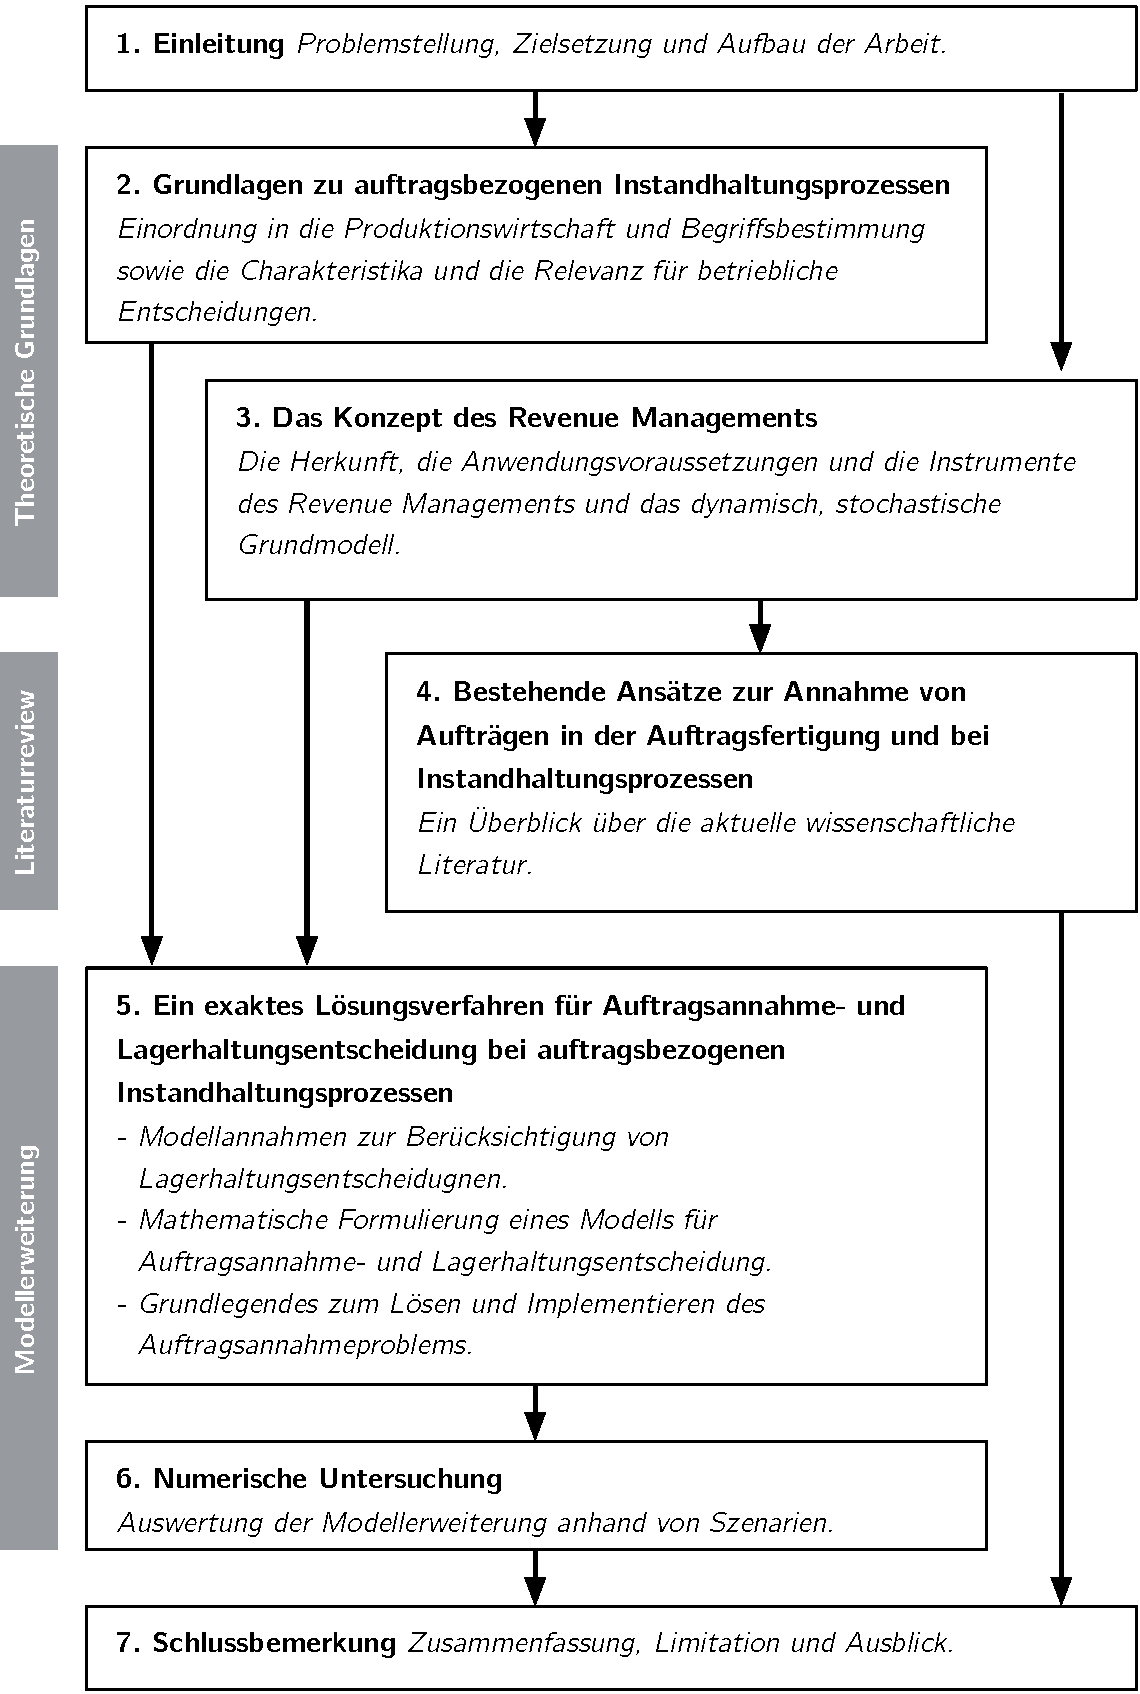
\includegraphics[width=140mm]{Bilder/Gliederung.pdf}
    \caption{Grafische Darstellung der Gliederung der Arbeit}  \label{Gliederung}
  \end{center}
\end{figure}


Der Aufbau der Arbeit ist in der Grafik \ref{Gliederung} dargestellt. In Kapitel 2 wird der Begriff \glqq auftragsbezogener Instandhaltungsprozess{\grqq} definiert und die theoretische Grundlagen zu diesem Begriff beschrieben. Der Begriff wird in die Produktionswirtschaft eingeordnet, sowie die Beschreibung der Charakteristika und der Relevanz für betriebliche Entscheidungen von auftragsbezogenen Instandhaltungsprozessen aufgeführt. In Kapitel 3 werden die theoretischen Grundlagen der Arbeit vervollständigt, indem das Konzept des RM zur Annahme von Aufträgen vorgestellt wird. In diesem Kapitel wird auf die Herkunft des Konzepts eingegangen, sowie auf die für das Konzept erforderlichen Anwendungsvoraussetzungen und auf die Instrumente. Des Weiteren ist in dem Kapitel die mathematische Modellformulierung des Grundmodells des Netzwerk RM dargestellt.

Im Anschluss wird in Kapitel 4 ein Literaturüberblick über bestehende Ansätze zur Annahme von Aufträgen der Auftragsfertigung und für Instandhaltungsprozesse aufgeführt. Kapitel 5 zeigt die Modellerweiterung des Netzwerk RM mit der Möglichkeit von Lagerhaltungsentscheidungen. Es werden im ersten Schritt die notwendigen Modellannahmen zur Berücksichtigung von Lagerhaltungsentscheidungen beschrieben und im Anschluss die mathematische Modellformulierung des Modells für Auftragsannahme- und Lagerhaltungsentscheidungen formuliert. Abschließend wird auf das Verfahren und auf den verwendeten Algorithmus zum exakten Lösen des Auftragsannahmeproblems eingegangen. Kapitel 6 zeigt die umfangreiche numerische Untersuchung der vordefinierten Szenarien und die Auswertung der optimalen Politik. Im letzten Kapitel sind die Schlussbemerkungen dieser Arbeit dargestellt. Es handelt sich dabei um eine Zusammenfassung der Ergebnisse der vorliegenden Arbeit, eine Beschreibung der Limitation des Modells und um einen Ausblick für nachfolgende Forschung.